
\chapter{Data}
\label{sec:Head Load Data}


Since the heat load image data was taken from real experiments, the data set is not uniform in the distribution of $\bar{\iota}$ values, which is shown in figure /ref{}. This means the distribution the network is attempting to learn is not uniform, or more explicitly, it's multimodal. This is a common problem in machine learning and is often addressed by using a loss function that is robust to multimodal distributions. The loss function used in this case is the mean squared error (MSE). The MSE is a common loss function for regression problems, but it is not entirely robust to multimodal distributions. This was address by M. Blatzheim et al. \cite{Blatzheim_2018} by using simulated input data that provided a continuos extension to the output distribution.

\begin{figure}[htb]
	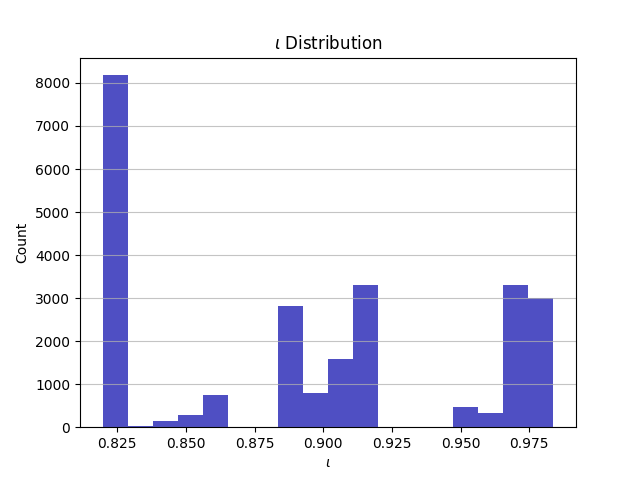
\includegraphics[width=\textwidth]{images/iota-dist.png}
	\caption{Distribution of simulated $\bar{\iota}$ values in the data set.}
	\label{fig:data:iota_dist}
\end{figure}

In an attempt to resolve this issue the distributions of the training, validation, and test sets were chosen to be as uniform as possible. This was challenging because the data is broken up into 42 different runs, or "shots". Each shot will have highly correlated data so mixing data from shots that are included in the test and validation set could serve to pollute the metrics used to evaluate overfitting or hyperparameter tuning.